\Chapter{Fejlesztői környezet}

Az OpenTTD már a kezdetlegi fázisaitól lehetővé tette azt, hogy a felhasználók saját AI-t fejleszthessen a játékhoz. Ennek a helyzetnek az előteremtésére a játék fejlesztői csapata létrehoztak egy API-t amit a Squirrel nyelv használatával elérést ad a játék back end-jéhez. Mivel a játék forrása tartalmaz egy fordítót, így a felhasználónak csak egy szövegszerkesztőre van szüksége az AI fejlesztéséhez.

\Section{A Squirrel programozási nyelv}

Az OpenTTD-hez készült kiegészítő szkriptek, AI-ok, módosítások nyelve a Squirrel \cite{squirrel}. A Squirrel egy egyszerű szkriptnyelv, aminek a szintaktikája sokban hasonlít a C++-ra. Legfőképpen két oka volt annak, hogy ezt a nyelvet választották a játék készítői. Elsősorban, sokban hasonlít a C++-ra, ami a fő nyelve a játék teljes forráskódjának. Másodsorban pedig, a Squirrel egy magas szintű,  imperatív, objektum orientált programozási nyelv, ami olyan célokkal lett megalkotva mint, egyszerű szkriptelés, alacsony memória használat és képesség a valós idejű programokkal való működésre, mint amilyenek a játékok is.

Ahogy korábban ez említésre került, a szintaktika főképpen C++-ra vagy C/Java-ra hasonlít, azonban a teljesítménye és implementációja inkább tükrözi a Python-t, JavaScript-et és Lua-t. A Lua több helyen is használt program, mint például az Adobe Photoshop Lightroom, MySQL Workbench, VLC media player és még sok más. Játékokban való alkalmazására példa a Far Cry és a Civilization V \cite{ierusalimschy2006programming}.

A Lua-hoz képest a Squirrel kevésbé elterjedt nyelv, és kevesebb eredményt is tud felmutatni, azonban néhány példát mindenképpen érdemes említeni a használatára ismertebb játékokban, úgy mint Left 4 Dead 2, Portal 2, GTA IV Multiplayer Mod és Counter Strike: Global Offensive.

A Squirrel nyelv főbb tulajdonságai:
\begin{itemize}
	\item delegáció,
	\item osztályok és öröklődés,
	\item magasabb rendű függvények,
	\item érvényességi terület (\textit{scope}),
	\item generátorok,
	\item kivételkezelés,
	\item rekurzió,
	\item automata memória kezelés.
\end{itemize}

Példa Sqirrel kódra:
\begin{cpp}
class Osztaly
{
  constructor(valt1,valt2)
  {
    // Konstruktor kódja
  }
  //változó definíciók
  local szoveg = "Ez egy szöveg";
  local szam = 10;
  local tomb = [0, "szöveg", [2.0, "tömb"]];
}
// Saját függvény definíció
function Osztaly::areaOfCircle(radius) {
  return (PI * radius * radius);
}
// Függvényhívás
local terulet = areaOfCircle(10);
\end{cpp}

A Squirrel egy dinamikusan típusos nyelv, ami azt jelenti, hogy a változók definiálásakor nem kell megadnunk az adott változó típusát, hanem a fordító azt automatikusan észleli és hozzárendeli. Azonban a futási idő alatt egy változó típusa változhat. Például egy integer változót ha szorzunk egy \texttt{float}-tal a kapott értékünk \texttt{float} típusú lesz.

A Squirrel-ben kétféle változót különböztetünk meg hatókör szerint. Az egyik a \texttt{local} a másik a \texttt{global} változó. Lokális változókat a \texttt{local} kulcsszóval tudunk definiálni, aminek a hatásköre az adott programrész lesz. Ezzel szemben a globális változókat általában a program gyökerében szokás definiálni. Fontos megjegyezni, hogy \texttt{global} kulcsszó nem létezik a nyelv szintaktikájában. A gyökérben definiált globális változóknál nem kell kulcsszót használnunk, azonban ha egy osztályon belül tesszük ezt meg a \texttt{::} hatókörfeloldó operátort kell használnunk. A változóknak nem szükséges memóriát allokálni, ezt a beépített memóriakezelő elvégzi helyettünk, valamint a deallokációt is.

\begin{cpp}
// Egy globális változó, kezdeti értékkel
aGlobalVariable <- 42.0;

// Globális változó egy osztályon kívül definiálva
::aGlobalVariable <- 42.0001;
\end{cpp}

A korábban felsorolt funkciói miatt a Squirrel egy nagyon rugalmas és egyszerűen implementálható eszköz, ami tökéletes egy játékhoz való API elkészítéséhez. A további előnyök, ami miatt az OpenTTD fejszeltői a Squirrel mellett döntöttek a C++ helyett az AI támogatáshoz a következőkben foglalhatók össze \cite{wisniewski2011artificial}.
\begin{itemize}
	\item Beépített multi-platform támogatás.
	\item A C++-ban írt AI-ok teszteléséhez az egész játék kódjának az újbóli összeállítására lett volna szükség.
	\item C++-ban a hibák az egész játék összeomlásához vezetnek, de Squirrel-ben a hibák a játékban futtatott virtuális gépen belül maradnak, ami legrosszabb esetben is csak az AI leállásához vezethet.
\end{itemize}

Érdemes megemlíteni, hogy a C++-hoz képest a Squirrel sebessége rosszabb, azonban ebben az alkalmazás módban kevésbé észrevehető. A legfőbb ok, ami miatt a játék szempontjából hasznos a Squirrel használata, az a biztonság és a hordozhatóság. Mindez ahhoz vezetett, hogy a játékhoz készült NoAI keretrendszer, amiről a későbbiekben részletesen is beszélünk, szintén a Squirrel nyelvben készült, ami ilyen formában támogatja az AI-ok működését.

Ahhoz, hogy Squirrel programot készítsünk, csak a Squirrel-re, és egy szövegszerkesztőre van szükségünk. Az előbbi a Squirrel weboldaláról letölthető. Az utóbbi pedig bármilyen fejlesztői környezet, vagy egyszerű szövegszerkesztő lehet. Az AI fejlesztése alatt a \textit{Visual Studio Code}-ot használtam \textit{Squirrel Language Supports} kiegészítővel, ami hozzáad a környezethez szövegkiemelést, néhány alapvető automata kitöltést és formázási lehetőségeket.

\Section{NoAI Keretrendszer}

A korábban fejlesztett, és jelenleg támogatott AI-ok mind a NoAI Framework nevű keretrendszerre épülnek. Egy másik lehetőség lenne egy AI megvalósítására a játékon belül a játék forráskódjának szerkesztése és annak újrafordítása, azonban a keretrendszer által adott egyszerűsítések jelentősen a háttérbe szorítják ezt az opciót. Amellett hogy ez sokkal bonyolultabbá tenné az AI implementálását, az elérhetőségét is korlátozná.

Ahogyan az korábban említésre került, az OpenTTD játék forráskódja nyílt, és a hozzá tartozó, felhasználók által készített szkriptek nagy része is az. A legtöbb az Általános Nyilvános Licenc (GNU) 2.0-ás vagy 3.0 változata alatt érhetőek el. Emiatt a fejlesztés megkezdése előtt két lehetőségünk van, az egyik egy AI megvalósítása teljesen a semmiből, vagy pedig egy már létező AI kódjának az átformázása a mi céljainkra, vagy esetleg már létező kódrészletek használata.

A keretrendszer részeként érdemes megemlíteni a játékhoz elérhető előre készített könyvtárakat. Néhány egyszerű, de fontos elemet tartalmaznak, amelyek közül a saját megvalósítás alatt használunk is. Ilyenek például a különböző útvonalkereső algoritmusok, amelyek út vagy vasútvonalakat tudnak létrehozni adott pontok között. A fejlesztő nincs ezeknek az elemeknek a használatára kötelezve, saját implementációt is készíthet egy útvonalkereső algoritmushoz.

\Section{NoAI API}

Ahogyan az korábban említve volt, a játék egy egészen bőkezű API-val rendelkezik, aminek a segítségével elérhetőek lesznek a fejlesztő számára azok a funkciók és információk, mint amik egy felhasználónak is elérhetőek a játék közben. Értve itt például a pálya állapotának lekérdezését, vagy utak építését. Minden funkció különböző osztályokba van rendezve, a szerint, hogy milyen feladatot lát el. Például az \texttt{AIStation} osztályban találunk olyan függvényeket, amelyekkel egy állomáshoz kapcsolódó információkat tudunk lekérdezni, vagy módosítani.

A különböző funkciók mellett az API felel a különböző AI-ok ütemezéséért is a játék futása alatt. Ugyanis a játék futása közben, egy vagy több AI-nak a játék időközönként futási időt ad, amikor a megírt programkód ténylegesen lefut. Ez a játékban egy \textit{round-robin} módszerű ütemezővel van megoldva, vagyis a vezérlés először a játéknál van, aztán több AI esetén, először az egyik kap időt parancsok végrehajtására, aztán pedig egy másik, amíg mindegyik sorra nem jut. Ezután a folyamat elölről kezdődik, így biztosítva, hogy a futási idő egyenletesen legyen elosztva.

Az \texttt{AIController} egy osztály, amivel már a minimális AI elkészítése során is találkozhatunk, ugyanis, a \texttt{main.nut}-on belül található osztályunknak az API ezen osztályából kell leszármaznia ahhoz, hogy a \texttt{Start()} függvényt meg tudjuk hívni az AI indításakor. Valamint, ezen keresztül kérdezhetőek le információk a játék jelenlegi állapotáról.

A fejlesztő szempontjából hasznosak lehetnek az \texttt{AIError}, \texttt{AIEvent} és \texttt{AILog} osztályok. Ezek segítségével van lehetőség kommunikálni a játék konzoljába a program futásából különböző nyomkövetéshez hasznos üzeneteket, vagy az \texttt{AIError} segítségével észlelhetőek és lekérdezhetőek a hibák.

Az AI szempontjából több hasznos osztály is rendelkezésre áll, egyrészt az \\ \texttt{AICompany} és \texttt{AIAccounting}, amelyek a céggel kapcsolatos információk lekérdezésében és változtatásában, továbbá a cég pénzügyeinek a kezelésében segítenek.

Talán a legfontosabbak a megfelelő működés érdekében az \texttt{AIMap} és \texttt{AITile} osztályok. Ugyanis a játék különböző infrastruktúrák kiépítésére alapszik. Ahhoz pedig, hogy megfelelő infrastruktúrát tudjunk építeni, először is alaposan fel kell mérnünk a játék pályáját, amit az \texttt{AIMap} függvényeinek segítségével tehetünk meg. Amikor a térkép egy részét lekérdezzük vagy vizsgáljuk, eredményül \texttt{AITile} osztályú objektumokat kapunk vissza, amik a térképen megtalálható egyes mezőket jelölik. Ezeknek a mezőknek van számtalan tulajdonságuk amelyek megszabják, hogy hogyan jelenik meg a felhasználó számára egy adott mező. Például, van-e út a mezőn vagy a mező esetleg víz-e? Az \texttt{AIMap} rendelkezik még több olyan függvénnyel, amelyek a későbbiekben hasznosak lesznek az útvonalak tervezésénél. Ilyen például a \texttt{DistanceManhattan(TileIndex tilefrom, TileIndex tileto)} aminek a segítségével két mező közötti Manhattan távolságot tudjuk lekérdezni. Ezzel tudjuk adott mezők közötti legrövidebb távolságot is kiszámítani.

Egy egyszerű példa az API osztályainak működésére:
\begin{cpp}
function GetTilesDistance()
{
  local TileList = AITileList();
  TileList.AddTile= (23);
  TileList.AddTile = (142);
  local distanceBetweenTiles =
  AIMap.DistanceManhattan(TileList.Begin(), TileList.Next());
  return distanceBetweenTiles;
}
\end{cpp}
Ebben a függvényben létrehozunk egy üres Listát ami mező objektumok tárolására alkalmas. Hozzáadjuk a 23 és 142 indexű mezőket a listához. Ennek a műveletnek előfeltétele, hogy a 23-as és 142-es indexű mezők valós, létező mezők. Aztán a listán lépegetve kezdve az elejétől, az \texttt{AIMap} API osztályának \texttt{DistanceManhattan()} függvényével kiszámoljuk a két mező közötti Manhattan távolságot amit a függvényünk ad meg visszatérési értékként.

Ezen felül a különböző szállítású módokhoz kapcsolódóan is vannak megfelelő osztályok, mint \texttt{AIRoad}, \texttt{AIRail}. Az \texttt{AIRoad} osztály ad rendelkezésünkre minden olyan függvényt amelyekre az utakkal kapcsolatban szükségünk lehet, például utak építése, garázsok építése vagy különböző információk lekérdezése a mezőn lévő útról.

Az API részeként elérhető az \texttt{AIList} osztály is, ami egy láncolt lista szerűen képes tárolni különböző típusú elemeket. Ennek az osztálynak a függvényei kifejezetten hasznosnak bizonyultak a fejlesztés során, mivel ennek az osztálynak a további gyerekosztályai például az \texttt{AITownList} és \texttt{AITileList} gyakran használatba kerültek. Ezek olyan listák, amelyek adott esetben a pályán található városokat, vagy mezőket, attól függően milyen listáról beszélünk, tartalmazzák. Az adott elemekhez a listán belül tudunk értéket is rendelni. Bár ez a funkció csak integer típusokra korlátozott, így is sok helyen felhasználható, főleg a \texttt{Valuate()} használatával, amivel az egész listának egyszerre adhatunk értéket egy értékelőfüggvény segítségével. Így például egyszerűen eldönthetjük hogy a listában szereplő mezők közül melyek utak, mivel attól függően, hogy út-e vagy sem, a függvény ad az elemeknek egy 0 vagy 1 értéket.

\Section{Nyomkövetés}

Az AI tesztelésére a játékon belül van lehetőségünk. Minden alkalommal amikor elindítunk egy játékot, és legenerálódott a világ, valamint beállítottuk, hogy rivális cégként megjelenjen az AI-unk is, akkor minden alkalommal elölről indul az AI-unk futtatása. Az AI által generált hibák, üzenetek követésére két módszerünk van, az egyik a játék konzolja, amit a "0" gomb lenyomásával tudunk elérni egy játékon belül. Itt lehet parancsokat kiadni, amivel elindíthatjuk manuálisan is az AI-t, vagy leállíthatjuk. A másik opció pedig az "MI/Játékszkript nyomkövetés", amit a játék közben a felső eszköztár utolsó menüpontjában találunk. Ez az ablak \aref{fig:console}. ábrán látható. Ebben az ablakban jelennek meg a szövegek, amiket az \texttt{AILog.Info()} vagy \texttt{AILog.Error()} segítségével kiíratunk, így nyomon követhető hogy éppen mi is történik az AI-al. Emellett található itt egy gomb, amivel újra tudjuk tölteni az AI-t, és egy gombot amivel ugyan azt a menüt tudjuk a játék közben is elérni, mint amit a főmenüből az "MI/Játékszkript beállítások" alatt tudunk megnyitni.

Példa az API használatára a nyomkövetéshez:
\begin{cpp}
AILog.Info("Ez egy egyszerű szöveg");
AILog.Info("Ez szöveg egy adott változóval" + szam);
AILog.Error("Ez a szöveg pirosan jelenik meg az ablakban");
\end{cpp}

Abban az esetben, ha a programunk fordítás, vagy futás közben olyan hibába ütközik, amit nem kezeltünk le, egy részletes hibajelentést kapunk róla a nyomkövető ablakban, és a játék konzoljában is. Ez pontosan leírja, hogy melyik sor futása közben lépett fel a hiba, és az adott pillanatban a létező változóknak mi volt az értéke. Ez a funkció nagyon hasznos volt az AI fejlesztése közben, mivel jelentősen megkönnyítette a hibajavítás folyamatát, mert a Visual Studio Code-hoz használt Squirrel kiegészítő nem rendelkezett teljes szintaktikai hiba észleléssel, azonban az első futtatás után könnyen megtalálhatóak voltak az adott hibák.

\begin{figure}
	\centering
	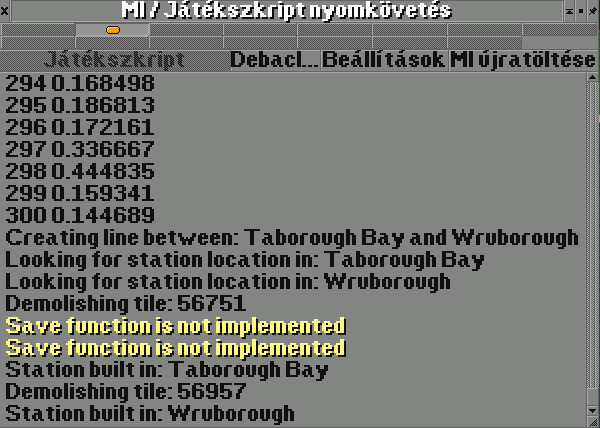
\includegraphics[width=\textwidth]{images/console.png}
	\caption{A játékon belül található nyomkövető ablak.}
	\label{fig:console}
\end{figure}

\Section{Minimális AI}

A következő szövegrész az OpenTTD szkript fejlesztői oldalán az AI-okra vonatkozó részének rövid összefoglalása \cite{noaidev}.

Azt mutatja be, hogy hogyan tudunk megvalósítani egy AI-t a játék keretein belül. Három dologra van szükségünk ahhoz hogy ezt létrehozzuk. Először is a játék mappáján belül található \texttt{ai} nevű mappában kell létrehoznunk egy mappát, szabvány szerűen az AI nevével. Aztán ebben a mappában 2 fájlra lesz szükségünk, mindkettő Squirrel nyelvű \texttt{.nut} kiterjesztésűnek kell lennie, az egyik \texttt{info.nut} a másik pedig \texttt{main.nut} néven kell létrehoznunk.

Az \texttt{info.nut} fájlban tudjuk megadni az általános információkat az AI-unkról, például a szerző nevét, az AI nevét, a játékban elérhető rövid leírását, a kód verziószámát és kiadási dátumát. Ebben az osztályban van lehetőségünk különböző beállítások definiálására is, amihez a felhasználó az egyik a játékban található menüpontban tud hozzáférni. Ahhoz, hogy a játék magjának is a tudtára adjuk, hogy ez egy AI a \texttt{RegisterAI()} nevű függvényt kell meghívnunk.

Példa az \texttt{info.nut} tartalmára:

\begin{cpp}
class MyNewAI extends AIInfo
{
  function GetAuthor()        { return "Newbie AI Writer"; }
  function GetName()          { return "MyNewAI"; }
  function GetDescription()   { return "An example AI"; }
  function GetDate()          { return "2007-03-17"; }
  function GetShortName()     { return "MYAI"; }
  function CreateInstance()   { return "MyNewAI"; }
}

/* Itt mondjuk meg a magnak hogy egy AI vagyunk */
RegisterAI(MyNewAI())
\end{cpp}

Ha ezzel készen vagyunk, a másik "\texttt{main.nut}" fájlban tudjuk az AI viselkedését meghatározni. Itt kell megadnunk a fő ciklusát az AI-nak, valamint egyéb osztályok és forrásfájlokra való hivatkozásokat. Az osztálynak néhány alapértelmezett funkciója van melyek a következőek:
\begin{itemize}
	\item \texttt{Start()} - Itt kapja meg a vezérlést az AI.
	\item \texttt{Save()} - Ezzel tudjuk lementeni az AI állapotát amikor a játékmenet mentése történik.
	\item \texttt{Load()} - A játék betöltésénél itt tudjuk betölteni a korábban lementett állapotát az AI-nak.
\end{itemize}

Ezek közül a függvények közül számunkra a \texttt{Start()} a legfontosabb, ugyanis, amikor elindítjuk az AI-t a játékon belül, ez a függvény fog meghívódni, és az itt megírt programrészek fognak lefutni. Éppen emiatt, ha azt szeretnénk, hogy a játék közben folyamatosan fusson az AI-unk, egy végtelen ciklusba érdemes belerakni a főbb parancsokat, amelyek ismétlődésével jön létre az AI játékmenete.
\begin{cpp}
class MyNewAI extends AIController
{
  function Start()
  {
    while (true) {
      AILog.Info("Tell the console we are running");
    }
  }
  function Save();
}

function MyNewAI::Save()
{
  return {};
}
\end{cpp}
Ahogyan a példában látható, a \texttt{MyNewAI} osztályunk leszármaztatja az API \\ \texttt{AIController} osztályát, ezáltal hozzáférést kap a beépített statikus függvényeinek használatára, mint a \texttt{Start()}, \texttt{Save()}, \texttt{Load()}. Az osztályon belül látható a \texttt{Save} függvény prototípusa, erre a Squirrel-en belül nincs szükség, de más programozási szabványban megszokott. Itt megfigyelhető, hogy kapcsos zárójelek helyett pontosvessző zárja a parancsot. Az alsó \texttt{Save()} függvény a valódi függvény definíciója a \texttt{Save}-nek. Mivel ez az osztály deklaráción kívül helyezkedik el, meg kell adnunk melyik osztályhoz tartozik, ezt a dupla kettőspont előtt tesszük meg.

Ahhoz, hogy ez az AI megjelenjen játék közben, még a főmenüben az "MI/Játékszkript beállítások" menüpont alatt be tudjuk állítani hány ellenfelet szeretnénk a játékunkban. Valamint azt is rögzíteni tudjuk, hogy az adott ellenfél melyik feltelepített AI legyen. Alapértelmezetten ez a beállítás véletlenszerű. Ha ezt beállítottuk, a játék indításakor a mi AI-unknak is meg kell jelennie a cégek között.

\Section{Hasonló implementációk}

Az OpenTTD játék kiegészítők nélküli verziójában nem található előre beépített gépi ellenfél, minden hasonló implementációt a játék közössége hozott létre. Ezek mind rendelkeznek a játék fórumán egy bejegyzéssel, valamint elérhetőek és letölthetőek a játékon belül, a fórumbejegyzésben megadott linkről, vagy pedig az ún. “BaNaNaS” repository-ból. Itt egyébként az összes a játékban elérhető szkriptek, fejlesztések, köztük a gépi ellenfelek listája megtalálható, mellette linkelve az adott tartalom fórumbejegyzését \cite{openttdbananas}. Ennek a tartalmát \aref{fig:bananas}. ábrán látható ablakban tudjuk elérni a játékon belülről. A meglévő AI-ok közül sok már nincs aktív fejlesztés alatt. A legtöbb fejlesztése a 2000-es évek végén kezdődött, aztán a 2010-es évek végére be is fejeződött. 2008 és 2017 között évente rendeztek AI bajnokságot, ahol különböző körökben egymásnak vetették az indulókat, és teljesítmény alapján értékelték azokat.

\begin{figure}
	\centering
	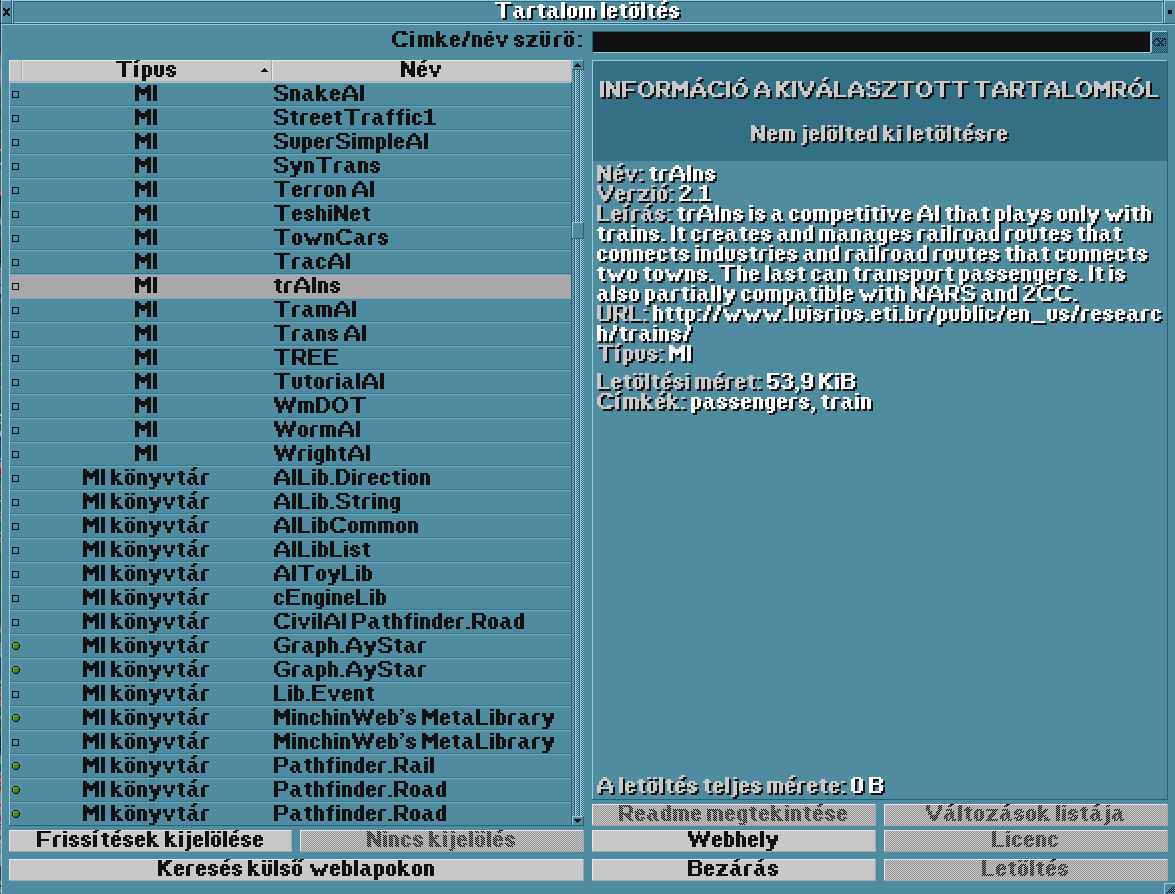
\includegraphics[width=\textwidth]{images/bananas.png}
	\caption{Játékszkriptek és AI-ok letöltése a játékon belől a BaNaNaS repositoryból.}
	\label{fig:bananas}
\end{figure}

A különböző AI-ok mind különböző céllal jöttek létre. Vannak, amelyek egyes szállítás módszer lehető legjobb megvalósítására fókuszálnak, például TrAIns (Vonatokra), RoadAI (közúti járművekre), Chopper (Légi közlekedésre). Ezek mellett vannak általánosak is, például az AdmiralAI, amelynek fókusza a lehető legtöbb funkció implementálása volt, vagy a SimpleAI ami szintén általános és több szállítási módszert is alkalmazó AI. Vannak olyan AI-ok is, amik lehet hogy nem a leghatékonyabban működnek, de van egy olyan tulajdonságuk, ami érdekessé tenné azt, például a PathZilla, ami gráfelmélet segítségével létrehozott úthálózatok építésére fókuszál, valamint többfajta útvonalkereső algoritmust alkalmaz.

Az AdmiralAI célja a játékhoz készített API legtöbb funkciójának kihasználása, valamint a változatos játékélmény biztosítása. Az utóbbit azzal próbálja meg elérni, hogy az AI minden szállítási módszert igyekszik alkalmazni. A mi szemszögünkből azért érdemes az AdmiralAI-al foglalkozni, mivel sok példát találhatunk a program forráskódjában, az API függvényeinek megvalósítására, valamint az AI felépítésére. A fájlszerkezet nagyon jól kitalált és felépített, minden összefüggő függvény, parancs, el van tagolva megfelelő osztályokba, mappákba, bár a kód értelmezése előzetes ismeretek nélkül elég nehézkes a kódhoz tartozó megjegyzésekkel együtt is. Az AI részletessége, és igényessége valamilyen szinten betudható adnak, hogy a készítője Thijs 'Yexo' Marinussen az OpenTTD, és az API egyik fejlesztője is egy személyben. Az AI sok inspirációt tud adni a sajátunk fejlesztéséhez, de előzetes ismeretekre van szükségünk az API-ról a megfelelő szintű megértéshez.

A PathZilla már sokkal érdekesebb megvalósítása egy AI-nak, mivel gráfelméleti algoritmusokat használ a városok összekötésére, és útvonalak megtervezésére \cite{openttdforum}. A PathZilla működéséről egy szemléltetést láthatunk \aref{fig:pathzilla}. ábrán. Először veszi a térképen található városok pozíciót, és ezek között létrehoz egy hálót Delaunay-háromszögeléses módszerrel. A kapott hálón megkeresi a legrövidebb utak fáját és a minimális feszítőfát, és a kettő összemosásával kapott gráf alapján köti össze az érintett városokat. Ez a működés szemléltetve van az AI fórum bejegyzésében egy rövid képsorozat formájában.

\begin{figure}
	\centering
	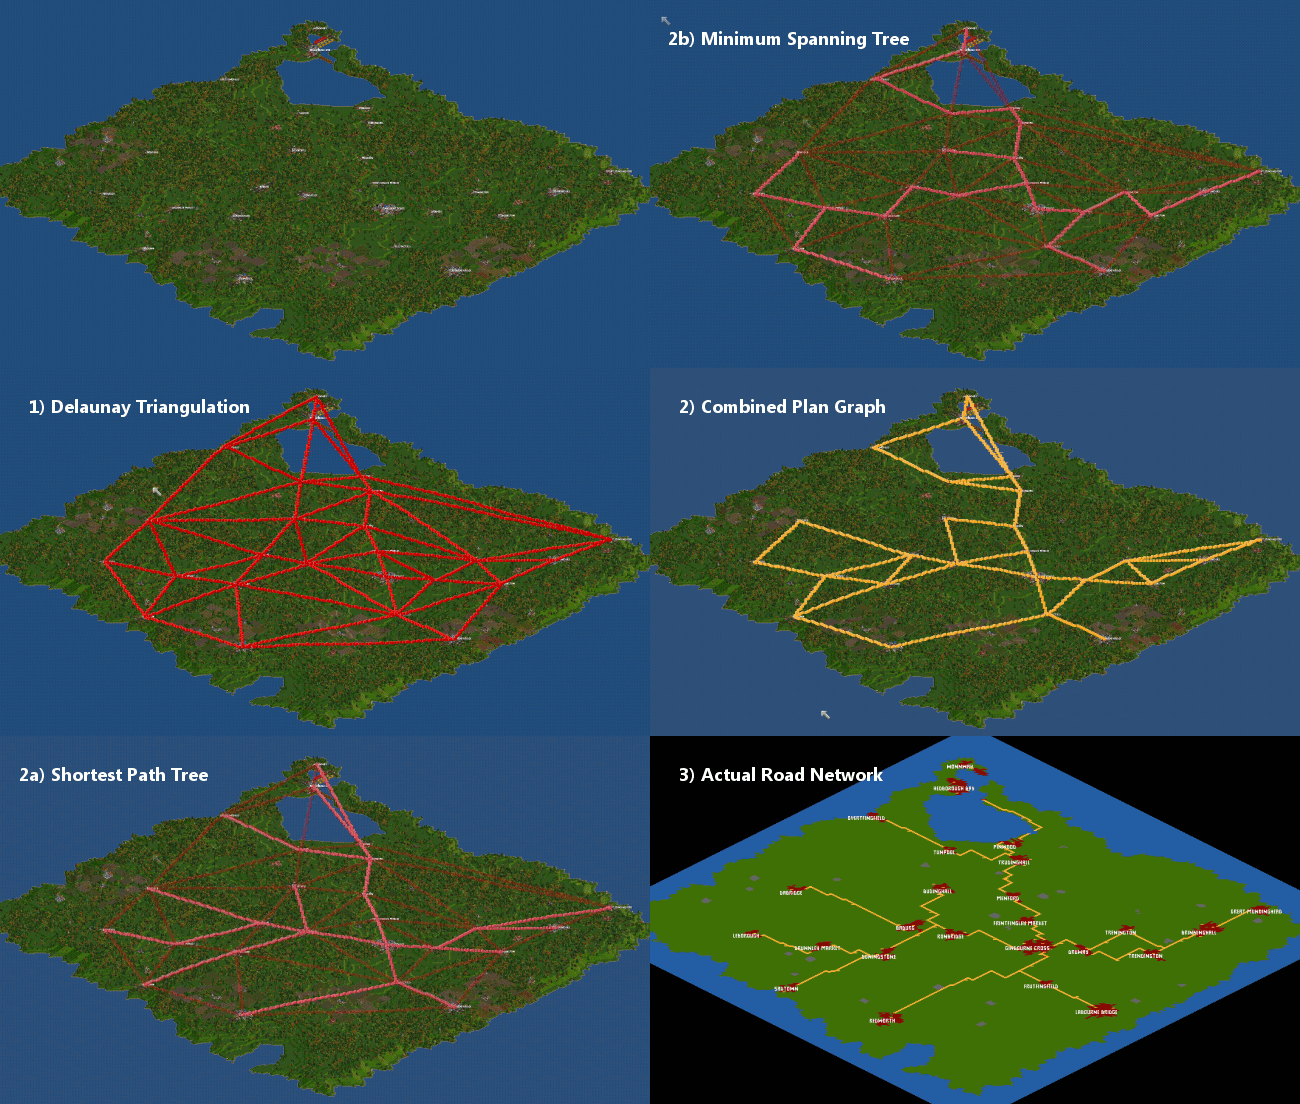
\includegraphics[width=\textwidth]{images/pathzilla.png}
	\caption{A PathZilla működésének szemléltetése. Forrás: \url{https://www.tt-forums.net/viewtopic.php?t=38645}}
	\label{fig:pathzilla}
\end{figure}

A TrAIns egy 2009-ben fejlesztett intelligencia, ami egy brazil egyetem két hallgatója által készült el, mint kutatói munka \cite{rios2009trains}. A céljuk az volt a projekttel, hogy egy olyan AI-t készítsenek, ami hatékonyan tud vasútvonalakat építeni és használni, ami akkoriban nem volt gyakori az AI-ok között, vagy nem hatékony megvalósítással rendelkezett. A korábbiakkal szemben, amelyek csak közvetlen összekötöttek állomásokat és egy vonat használta a pályát oda-vissza, ez az AI úgy épített vasútvonalakat, mint ahogyan azt egy játékos is tenné. Több vágányos vonalakat is épített, így lehetővé tette, hogy egy vonalon egyszerre több vonat is közlekedhessen, és ezek a vonalak keresztezni is tudják egymást. Ennek a segítségével képes egy célba több egymáshoz közeli forrásból árut elszállítani úgy, hogy a vonal nagy részét több vonat is használja egyszerre.

\Section{Saját stratégiák}

Az eddig megemlített AI-ok nagy része tudományos szempontból közelíti meg a játék problémáját. Ezzel szemben a saját megvalósításnál az én szempontom egy olyan AI készítése volt, amely többnyire a saját játékstílusom megvalósítása a számítógép erejének segítségével. Ez alatt azt értem, hogy a probléma megközelítése emberi szempontból történik, egy heurisztikus megoldásról van szó, azonban a tényleges döntéshozásokat már az AI fogja megtenni.

Amíg például a PathZilla esetében az útvonalak előre el vannak döntve különböző gráfoknak a segítségével és az útvonalak később kerülnek megépítésére, a játékos szemszögemből hatékonyabbnak tűnik, hogy ha csak néhány, arra érdemes város kerül összekötésre. Ezek általában a legnagyobb lakossággal rendelkező városok lesznek. Játék közben egy emberi felhasználó mire megvizsgálja a pálya jelenlegi helyzetét, és meghatározza két szomszédos városról hogy oda érdemes lehet-e egy buszvonalat létrehozni, ha az AI-nak meg tudjuk adni milyen szempontok alapján vizsgálja meg a pályát, lehet hogy ugyan arr, a döntésre, vagy annál jobbra tud jutni, mint a felhasználó, ráadásul rövidebb idő alatt.

Feltételezve, hogy a kiválasztott városok ideálisak, a buszmegálló kiválasztásának helye sem egyszerű döntési probléma. Amennyiben csak a térképet vesszük figyelembe, az AI sokkal alaposabban át tudja vizsgálni az adott területet, mint ahogyan arra egy játékosnak módja van.

A járművek kezelésének feladatát is átadva az AI-nak sokkal effektívebb tud lenni, mint egy átlagos felhasználó. Mivel egy új buszhálózathoz, egy játékos sokkal lassabban tudja felmérni egy vonalra küldendő szükséges buszoknak a számát, addig a program pár másodperc alatt döntésre tud jutni. A felhasználónak figyelnie kell a buszmegállóban várakozók számát, és ahhoz képest változtatni a buszokat, valamint az elöregedő buszok cseréjét is csak egyesével tudja elvégezni.
